\chapter{Introdução}


\setcounter{page}{1}    % set page to 1 again to start arabic count
\pagenumbering{arabic}


Capítulo 1 de Gonzalez, \textit{Digital Image Processing}~\cite{gonzalez2006image}.

%%%%%%%%%%%%%%%%%%%%%%%%%%%%%%%%%%%%%%%%%%%%%%%%%%%%%%%%%%%%
\section{O que é processamento de imagens}

\begin{easylist}
  & O que é uma imagem?
  && Uma matriz
  && Uma função
  && Esses conceitos podem ser generalizados para mais dimensões
  & Uma definição de processamento de imagens: processo em que tanto a entrada quanto a saída são imagens.
  && Essa definição não engloba, porém, processos como valor médio da imagem, extração de pontos característicos, alguns tipos de reconstrução 3D, aplicações de segurança que detectam atividades suspeitas, reconhecimento de gestos, reconhecimento de caracteres (OCR) e outras aplicações consideradas do campo de visão computacional.
  & Uma definição mais abrangente: processos de baixo, médio e alto nível em que tanto a entrada quanto a saída são imagens.
  && Baixo nível: envolve operações primitivas, de redução de ruído, aumento de contraste, aumento de nitidez (\textit{sharpening}), \textit{thresholding} etc. Nos processos de baixo nível, tanto a entrada quanto a saída são imagens.
  && Médio nível: envolve tarefas como segmentação (particionamento), redução dos objetos a uma descrição ou formato apropriado para processamento, classificação (reconhecimento) de objetos. A entrada são imagens, e a saída são atributos extraídos dessas imagens, como bordas, contornos, características ou classe de objetos individuais.
  && Alto nível: envolve atividades cognitivas associadas com a visão. Cognição envolve atividades como memória, compreensão, aprendizado, raciocínio, atenção, resolução de problemas e tomada de decisão.
\end{easylist}

%%%%%%%%%%%%%%%%%%%%%%%%%%%%%%%%%%%%%%%%%%%%%%%%%%%%%%%%%%%%
\section{Origens do processamento digital de imagens}

\begin{easylist}
  & 1920: \textit{Bartlane cable picture transmission system}, 5 tons de cinza.
  & 1929: idem, 15 tons de cinza.
  & 1948: invenção do transistor.
  & 1950 a 1960: invenção das linguagens de programação de alto nível, COBOL e Fortran.
  & 1958: invenção do circuito integrado.
  & 1964: primeira foto da Lua tirada de uma sonda.
  & 1968 a 1971: invenção dos primeiros microprocessadores, CADC, TMS1000, 4004.
  & 1969: invenção do CCD.
  & 1971: primeira tomografia computadorizada
\end{easylist}

%%%%%%%%%%%%%%%%%%%%%%%%%%%%%%%%%%%%%%%%%%%%%%%%%%%%%%%%%%%%
\section{Áreas que usam processamento digital de imagens}

\begin{easylist}
  & Medicina, astronomia, meteorologia, indústria, fotografia, editoração, segurança etc.
  & Técnicas de obtenção de imagem:
  && Eletromagnética: luz, radiação UV, radiação IR, raios X, raios gama, microondas.
  && Eletrônica: microscopia eletrônica.
  && Mecânica: ondas acústicas, ultrassom.
  && Sintética: computação gráfica, fractais.
\end{easylist}

%%%%%%%%%%%%%%%%%%%%%%%%%%%%%%%%%%%%%%%%%%%%%%%%%%%%%%%%%%%%
\section{Passos fundamentais no processamento digital de imagens}

\begin{easylist}
& Aquisição
&& Ao adquirir e salvar um conjunto de imagens, é preciso ter cuidado com o formato do arquivo e compressão usada. A depender do tipo de compressão, podem ocorrer perdas que comprometam o uso das imagens adquiridas. A Figura~\ref{fig:compress} mostra exemplos de artefatos de compressão. A Figura~\ref{fig:compress:25} foi obtida da compressão de~\ref{fig:compress:orig} em formato JPG com qualidade 25 usando o {\it software} GIMP. Os artefatos de compressão podem ser melhor observados em~\ref{fig:compress:orig:eye}. A Figura~\ref{fig:compress:12bit} foi obtida da compressão de~\ref{fig:compress:orig} pela redução da profundidade de cor, ou seja, ao invés de usar 8 bits, foram usados 4 bits por amostra, ou seja, um total de 12 bits por pixel. Esse efeito pode ser emulado no GIMP através do filtro {\it Posterize}. O efeito visual dessa perda de informação é conhecido como {\it color banding}.
& Melhoramento (\textit{image enhancement)}
& Restauração
& Processamento de cores
& \textit{Wavelets} e processamento multirresolução
& Compressão
& Processamento morfológico
& Segmentação
& Representação e descrição
& Reconhecimento de objetos
\end{easylist}


\def\WORIG{.45\textwidth}
\def\WDET{.525\textwidth}

\begin{figure}[!t]
  \begin{subfigure}{\WORIG}
    \centering
    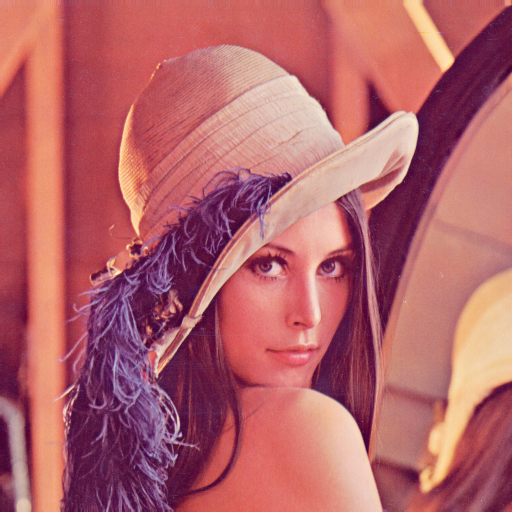
\includegraphics[width=1\textwidth]{images/01/lena_orig.png}
    \caption{\label{fig:compress:orig} Figura original.}
  \end{subfigure}
  \begin{subfigure}{\WDET}
    \centering
    
\includegraphics[width=1\textwidth]{images/01/lena_orig_eye.png}
    \caption{\label{fig:compress:orig:eye} Detalhe de (a).}
  \end{subfigure}
  
  \begin{subfigure}{\WORIG}
    \centering
    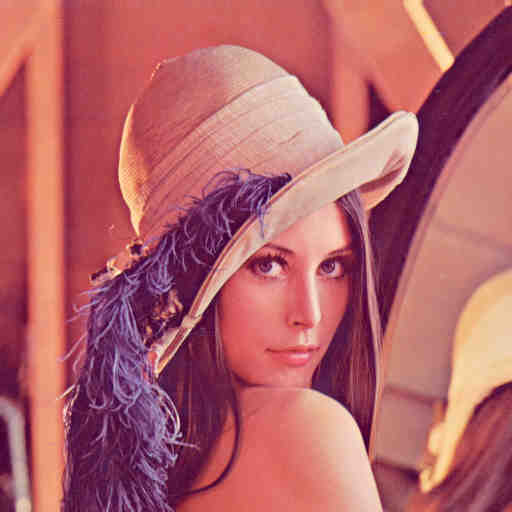
\includegraphics[width=1\textwidth]{images/01/lena_25.png}
    \caption{\label{fig:compress:25} Versão JPG.}
  \end{subfigure}
  \begin{subfigure}{\WDET}
    \centering
    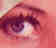
\includegraphics[width=1\textwidth]{images/01/lena_25_eye.png}
    \caption{\label{fig:compress:25:eye} Detalhe de (c).}
  \end{subfigure}

  \begin{subfigure}{\WORIG}
    \centering
    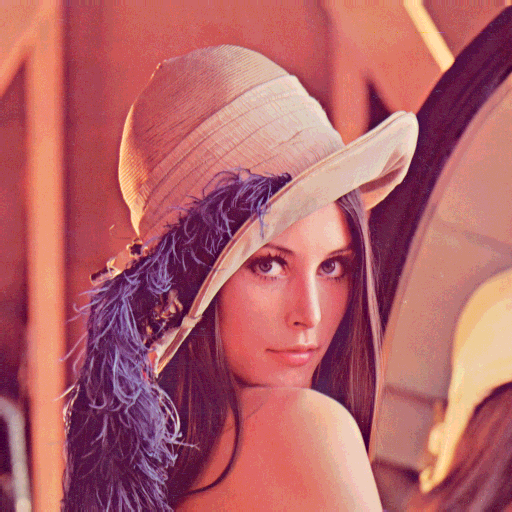
\includegraphics[width=1\textwidth]{images/01/lena_12bit.png}
    \caption{\label{fig:compress:12bit} Versão com 4 bits por amostra.}
  \end{subfigure}
  \begin{subfigure}{\WDET}
    \centering
    
\includegraphics[width=1\textwidth]{images/01/lena_12bit_eye.png}
    \caption{\label{fig:compress:12bit:eye} Detalhe de (e).}
  \end{subfigure}

  \caption{\label{fig:compress} Exemplos de artefatos de compressão.}
\end{figure}



%%%%%%%%%%%%%%%%%%%%%%%%%%%%%%%%%%%%%%%%%%%%%%%%%%%%%%%%%%%%
\section{Componentes de um sistema de processamento de imagens}

\begin{easylist}
& Sensores + \textit{hardware} especializado
& Computador + GPU
& Armazenamento em massa
& \textit{Software} de processamento de imagens
& Monitor de imagem
& Impressora
& Rede
\end{easylist}
